\subsection{Normalmapping}
\label{section:Normalmapping}

Um die visuelle Qualität eines Models zu erhöhen, muss detailliertere Modellierung erfolgen aus der eine höhere Anzahl von Dreiecken resultiert. 
Damit erhöht sich aber auch der Rechenaufwand für dieses Model. Ab einer bestimmten Grenze ist die gewonnene Qualität nur sehr gering, der Rechenaufwand aber um so größer. 
Um ein Model trotzdem mit einer höheren Auflösung darzustellen, wird ein Vorgang namens \textit{Normalmapping} verwendet. 
Dieser baut auf Lichtberechnungen auf. Ohne Licht gibt es keine zu erkennende verbesserte Qualität. Normalerweise hat jeder Vertex einen Normalenvektor und für einen Pixel wird er zwischen den drei Vertices interpoliert. 
Mit Normalmapping weist man jedem Pixel einen eigenen Normalenvektor zu. So ist es möglich, die Oberfläche so aussehen zu lassen, als würde sie rau mit kleinen Unebenheiten sein. Somit wird kein Rechenaufwand durch das Rendern vieler Dreiecke eines Meshes unnötig erzeugt.
Den Unterschied sieht man in \cref{img:Normalmapping}. Die Normalenvektoren werden in einer Textur gespeichert, sodass sie mit den normalen Texturen-Koordinaten verwendet werden können. Diese Textur wird im Material abgespeichert.

In einer Textur können die drei Werte rot, grün und blau, jeweils mit einem Wert von 0 bis 1, abgespeichert werden. Ein Normalenvektor hat drei Komponenten mit jeweils Werten von -1 bis 1. Daher muss dieser erst berechnet werden:

$ \overrightarrow{N} = 
\begin{pmatrix}
x \\ y \\ z
\end{pmatrix}
 = 2 \cdot \overrightarrow{C} - 1 = 
 \begin{pmatrix}
 2 \cdot r - 1 \\ 2 \cdot g - 1 \\ 2 \cdot b - 1
 \end{pmatrix}$
 
Der Normalenvektor $\begin{pmatrix}
	0 \\ 0 \\ 1
\end{pmatrix}$ zeigt direkt vom Model weg, daher sind Normalmaps auch immer sehr bläulich. Der meiste Anteil des Normalenvektors liegt in der Z-Komponente. Ein Beispiel einer Normalmap ist in \cref{img:Normalmap} zu sehen. Man kann diesen Vektor nicht direkt verwenden, da er im \textit{Tangent Space} definiert ist. 
Dies bedeutet, dass er relativ zu dem zugehörigen Dreieck steht.
Man benötigt zudem einen Normalenvektor im \textit{Object Space}, also relativ zu dem Model. 
Zur Umwandlung wird eine 3x3 Matrix benötigt, die aus drei verschiedenen Vektoren des Tangent-Space gebildet wird. 
Es können hierbei drei beliebige nicht linear abhängige Vektoren verwendet werden. Man bemerkt schnell, dass, wenn alle drei orthogonal zueinander verlaufen, es einfacher und effizienter ist, die Matrix zu erstellen. 
Der erste Vektor ist der Standardnormalenvektor jedes Vertex. Hinzu kommt noch ein Tangentenvektor jedes Vertex. Dieser befindet sich ebenfalls im \ac{VBO} des Meshes, wie in \cref{table:VertexAufbau} abgebildet. Der dritte Vektor ist der Bitangentenvektor und kann mittels Kreuzprodukt aus den Standardnormalenvektor und dem Tangentenvektor berechnet werden. Es ist nötig alle drei Vektoren zu normalisieren, bevor die Matrix erstellt wird.

Gegeben ist der Normalenvektor $\overrightarrow{N}$ und der Tangentenvektor $\overrightarrow{T}$

Die normalisierten Vektoren: $\overrightarrow{N_{0}} = \dfrac{\overrightarrow{N}}{|\overrightarrow{N}|}$\qquad	$\overrightarrow{T_{0}} = \dfrac{\overrightarrow{T}}{|\overrightarrow{T}|}$

Der Bitangentenvektor: $\overrightarrow{B} = \overrightarrow{N_{0}} \times \overrightarrow{T_{0}}$\qquad	$\overrightarrow{B_{0}} = \dfrac{\overrightarrow{B}}{|\overrightarrow{B}|}$

Die Matrix: $M =  \begin{pmatrix}
T_{0x} & B_{0x} & N_{0x} \\
T_{0y} & B_{0y} & N_{0y} \\
T_{0z} & B_{0z} & N_{0z} \\
\end{pmatrix}$

Diese Matrix wird für erhöhte Leistung im Vertex-Shader erstellt und daraufhin dem Fragment-Shader übergeben. In diesem muss der Normalenvektor aus der Normalmap geladen werden. Dafür werden die gleichen Texturkoordinaten (wie bei der Color-Texture) verwendet und mit dieser Matrix multipliziert.

\begin{figure}
	\begin{center}
		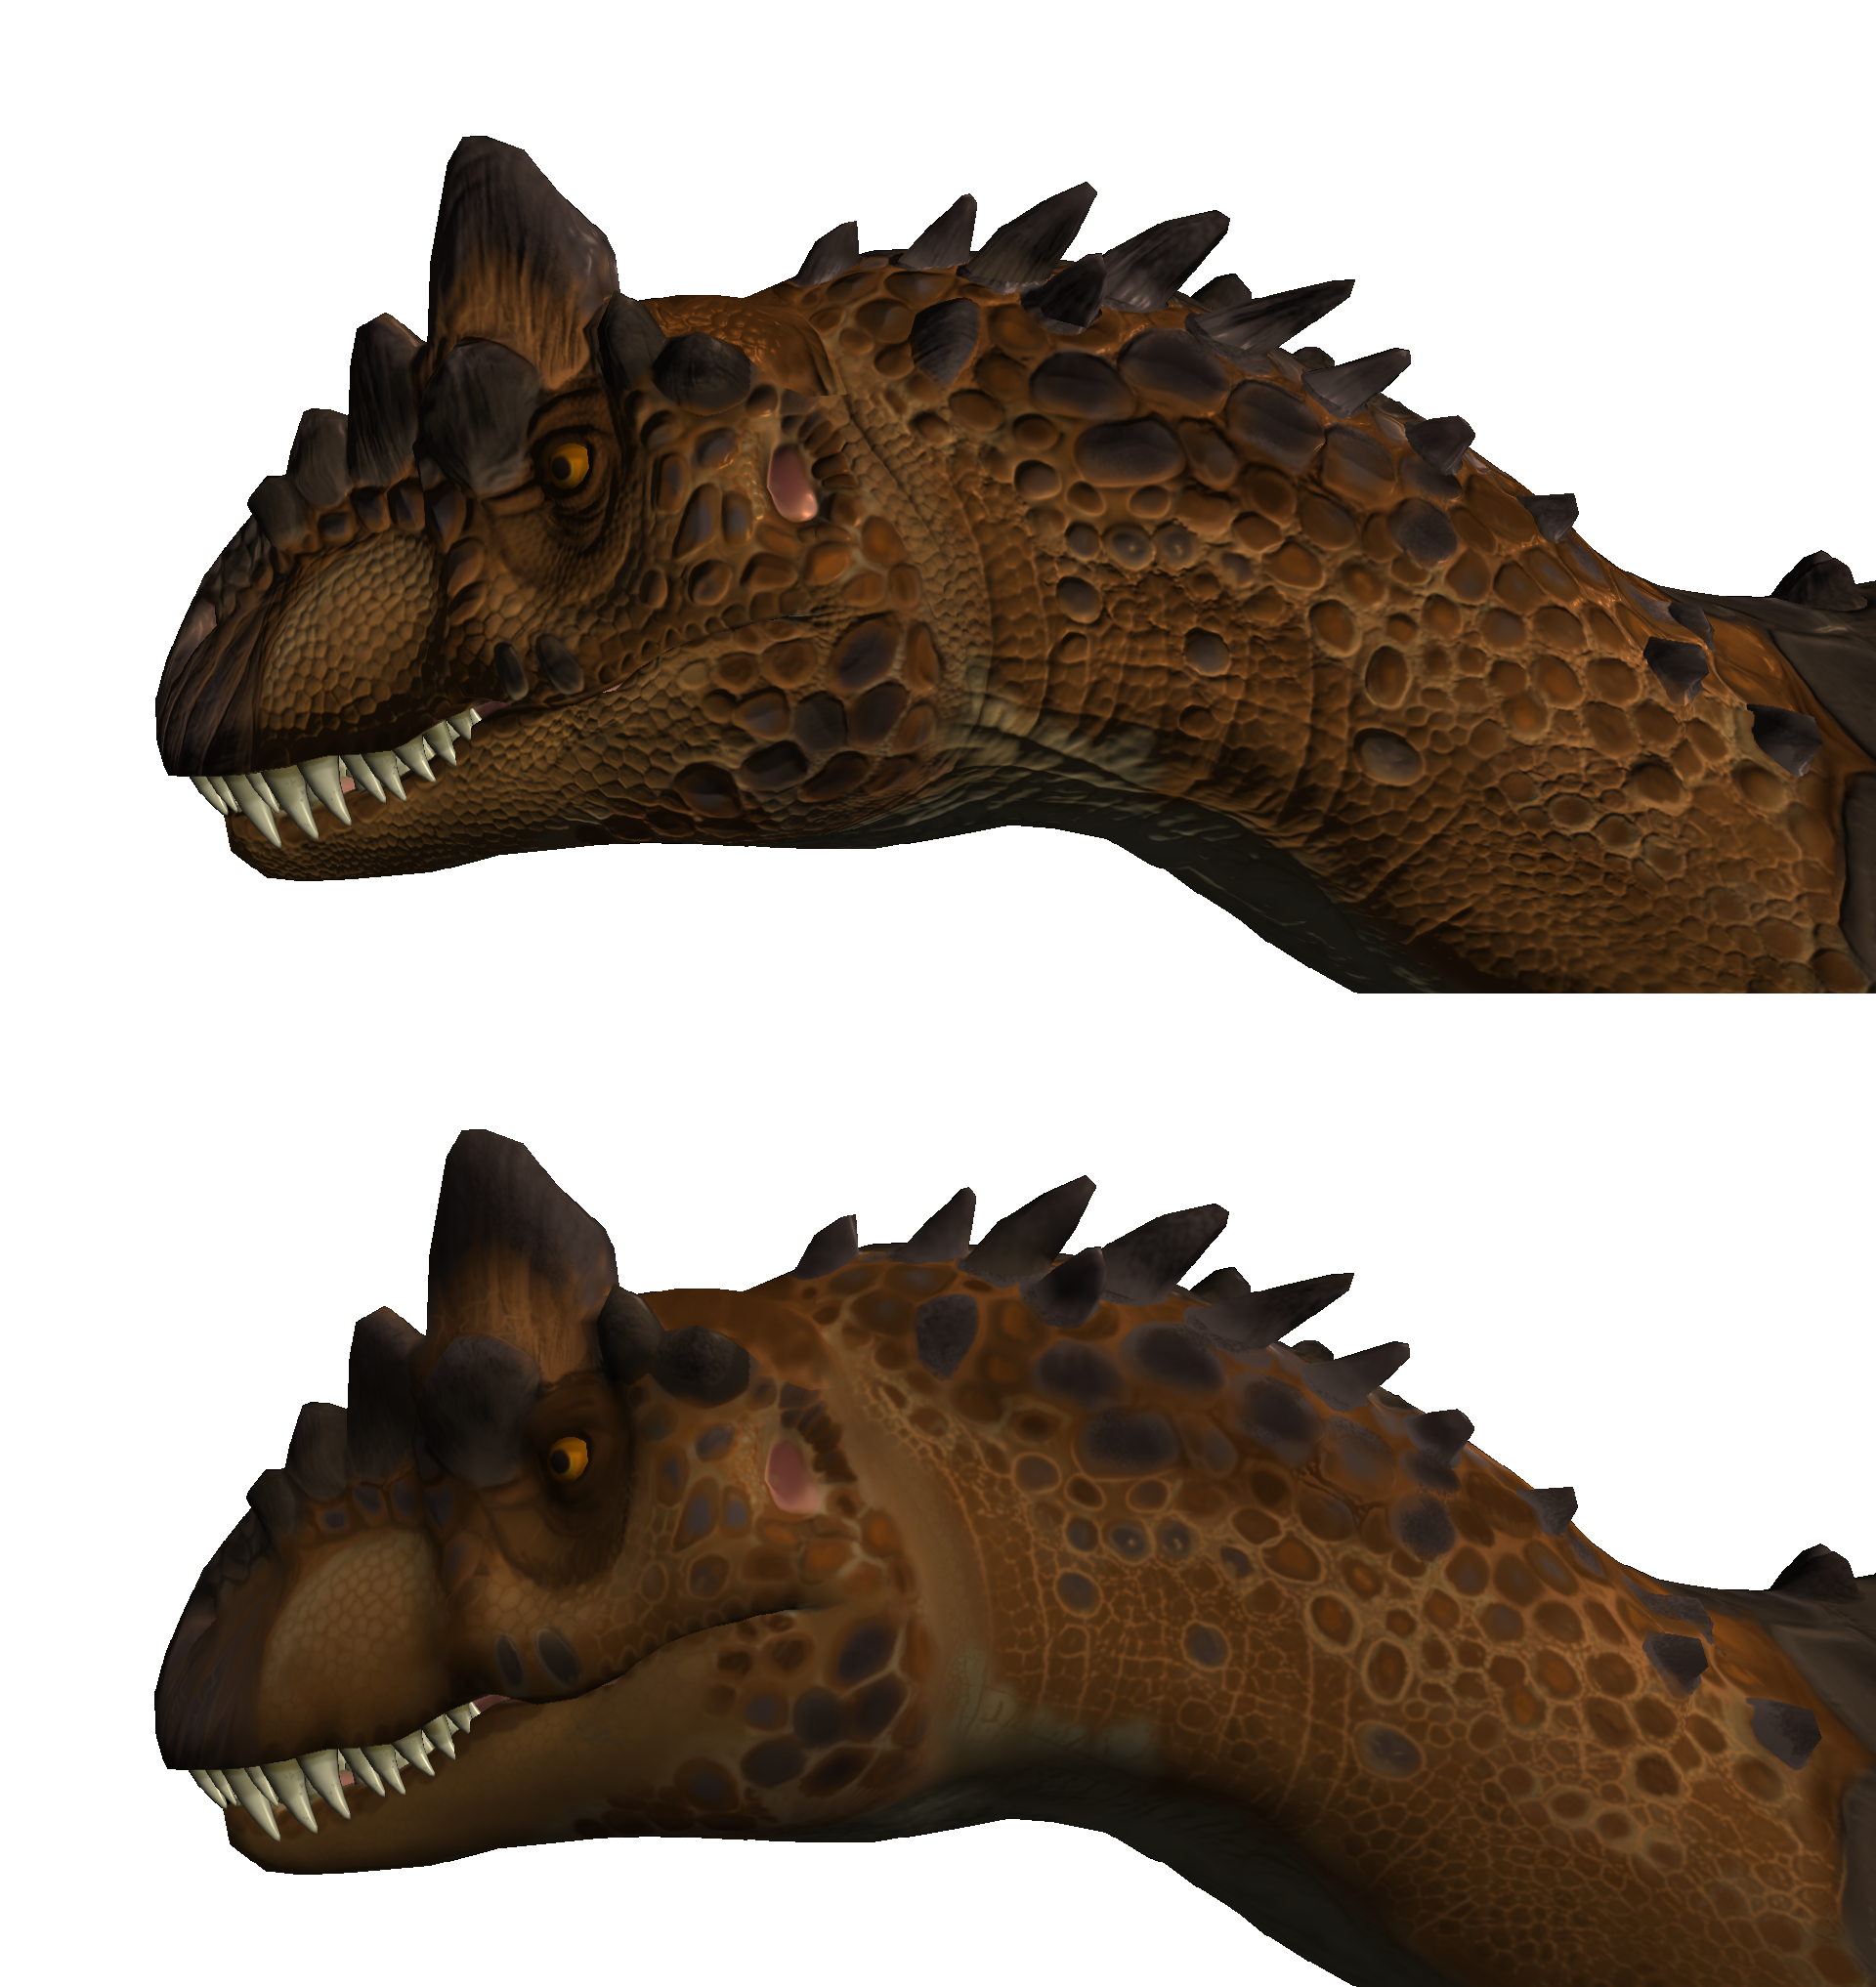
\includegraphics[width=0.5\textwidth]{02theorie/Normalmapping.png}
		
		Oben: mit Normalmapping, Unten: ohne Normalmapping
		
		Model: Allosaurus aus dem Spiel "`Ark: Survival Evolved"
		
		\caption{Normalmapping Beispiel}
		\label{img:Normalmapping}
	\end{center}
\end{figure}
\begin{figure}
	\begin{center}
		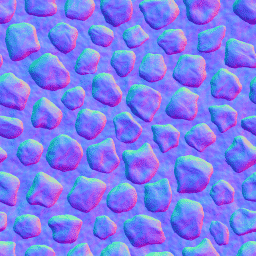
\includegraphics[width=0.4\textwidth]{02theorie/normalmap.png}
		
		Eine Beispiel Normalmap
		
		Quelle: http://www.bencloward.com/images/tutorial\textunderscore normals07.gif
		
		\caption{Normalmap Beispiel}
		\label{img:Normalmap}
	\end{center}
\end{figure}